%%%%%%%%%%%%%%%%%%%%%%%%%%%%%%%%%%%%%%%%%%%%%%%%%%%%%%%%%%%%%%%%%%%%%%%%%%%%
%%%  4th International Digital Libraries for Musicology workshop (DLfM)  %%%
%%%  Modeling the Complexity of Music Metadata in Semantic Graphs        %%%
%%%%%%%%%%%%%%%%%%%%%%%%%%%%%%%%%%%%%%%%%%%%%%%%%%%%%%%%%%%%%%%%%%%%%%%%%%%%

\documentclass[sigconf]{acmart}

\usepackage{booktabs} % For formal tables
\usepackage{listings}
\usepackage[neverdecrease]{paralist}

\newcommand\figref{Figure~\ref}
\newcommand\tabref{Table~\ref}
\newcommand\smallsc[1]{\textsc{\small{#1}}}

\makeatletter
\newcommand\footnoteref[1]{\protected@xdef\@thefnmark{\ref{#1}}\@footnotemark}
\makeatother

% Copyright
%\setcopyright{none}
%\setcopyright{acmcopyright}
%\setcopyright{acmlicensed}
%\setcopyright{rightsretained}
%\setcopyright{usgov}
%\setcopyright{usgovmixed}
%\setcopyright{cagov}
%\setcopyright{cagovmixed}

% DOI
%\acmDOI{10.475/123_4}

% ISBN
\acmISBN{978-1-4503-5347-2}

%Conference
\acmConference[DLfM'17]{4th International Digital Libraries for Musicology workshop}{October 2017}{Shanghai, China} 
\acmYear{2017}
\copyrightyear{2017}
%\acmPrice{15.00}

%%%%%%%%%%%%%%%%%%%%%%%%%%%%%%%
%%%  Beginning of document  %%%
%%%%%%%%%%%%%%%%%%%%%%%%%%%%%%%

\begin{document}
\title{Modeling the Complexity of Music Metadata in Semantic Graphs for Exploration and Discovery}

\author{Pasquale Lisena,~~~Rapha\"el Troncy}
\affiliation{%
  \institution{EURECOM}
  \city{Sophia Antipolis} 
  \state{France} 
}
\email{{lisena, troncy}@eurecom.fr}

\author{Konstantin Todorov, Manel Achichi}
\affiliation{%
  \institution{LIRMM, University of Montpellier}
  \city{Montpellier} 
  \country{France} }
\email{{todorov,achichi}@lirmm.fr}


% The default list of authors is too long for headers}
\renewcommand{\shortauthors}{P. Lisena et al.}
\renewcommand{\shorttitle}{Modeling the Complexity of Music Metadata in Semantic Graphs}

%%%%%%%%%%%%%%%%%%
%%%  Abstract  %%%
%%%%%%%%%%%%%%%%%%

\begin{abstract}
Representing and retrieving fine-grained information related to something as complex as music composition, recording and performance is a challenging activity. This complexity requires that the data model enables to describe different outcomes of the creative process, from the writing of the score, to its performance and publishing. In this paper, we show how we design the DOREMUS ontology as an extension of the FRBRoo model in order to represent music metadata coming from different libraries and cultural institutions and how we publish this data as RDF graphs. We designed and re-used several controlled vocabularies that provide common identifiers that overcome the differences in language and alternative forms of needed concepts. These graphs are interlinked to each other and to external resources on the Web of Data. We show how these graphs can be walked through for designing a web-based application providing an exploratory search engine for presenting complex music metadata to the end-user. Finally, we demonstrate how this model and this exploratory application is suitable for answering non-trivial questions collected from experts and is a first step towards a fully fledged recommendation engine.
\end{abstract}

%
% The code below should be generated by the tool at
% http://dl.acm.org/ccs.cfm
% Please copy and paste the code instead of the example below. 
%
\begin{CCSXML}
<ccs2012>
<concept>
<concept_id>10002951.10003317.10003318.10011147</concept_id>
<concept_desc>Information systems~Ontologies</concept_desc>
<concept_significance>500</concept_significance>
</concept>
<concept>
<concept_id>10002951.10003317.10003331.10003336</concept_id>
<concept_desc>Information systems~Search interfaces</concept_desc>
<concept_significance>500</concept_significance>
</concept>
<concept>
<concept_id>10002951.10003317.10003371.10003386.10003390</concept_id>
<concept_desc>Information systems~Music retrieval</concept_desc>
<concept_significance>500</concept_significance>
</concept>
<concept>
<concept_id>10002951.10003260.10003309.10003315</concept_id>
<concept_desc>Information systems~Semantic web description languages</concept_desc>
<concept_significance>300</concept_significance>
</concept>
</ccs2012>
\end{CCSXML}

\ccsdesc[500]{Information systems~Ontologies}
\ccsdesc[500]{Information systems~Search interfaces}
\ccsdesc[500]{Information systems~Music retrieval}
\ccsdesc[300]{Information systems~Semantic web description languages}

\keywords{Ontology, FRBRoo, Music Metadata, Linked Data, Data Interlinking}

%\acmBadgeR{artifacts_available}

\maketitle

\setdefaultleftmargin{0.5cm}{1.5cm}{}{}{}{}

%%%%%%%%%%%%%%%%%%%%%%%%%
%%%  1. Introduction  %%%
%%%%%%%%%%%%%%%%%%%%%%%%%

\section{Introduction}\label{sec:introduction}
Music metadata can be very complex. Metadata about a well-known masterpiece such as the \textit{Moonlight Sonata} can include a description of its composition by Beethoven, its scores in the handwritten or printed version, some interpretations by pianists, the orchestrations and arrangements. Performances, recordings, music albums can also be described and attached to this work. Numerous actors are involved in this media production chain: composers, performers with their own different roles, conductors, etc. An even more challenging tasks consist in describing jazz and ethnic music for which the performance plays a central role. In jazz, each improvisation can be considered as a creation event of a new expression, whose the performer is the author. In ethnic music, the absence of a score and a composer, as in classical western music, requires a different way of describing it.

Libraries have plenty of structured information that is currently encoded in different formats such as relational tables, XML, CSV and very specialized ones like MARC and its variants. This heterogeneity is not satisfactory for different reasons. The structure of the data is often guided by a set of arbitrary rules, internal to each institution and with non-explicit semantics, making the understanding of the model hard. Furthermore, some musical works are described by different catalogs with complementary and overlapping metadata. Discovering duplicates and performing a reconciliation and interconnection of the data will produce enriched information that will combine the knowledge coming from different data sources. In its current state, music metadata has little chances of effortless and automatic reconciliation and linking. Finally, these formats are not ready to be directly consumed by applications for visualization, exploration and recommendation. They require significant parsing efforts and semantic interpretation which deter their full potential usage. We observe that, alongside advanced search interfaces allowing to select subset of works with specific properties, musical institutions are constantly more interested in automatic support for the editorial work of making the programme for a concert or a musical playlist for a radio show. This help can come from a recommendation system that shall reveal, starting from a seed, the best choices to listen among the huge amount of data available, based on relatedness criteria more then on a personalisation aim.

In this paper, we present our current results in harmonizing the musical data coming from three leading cultural institutions in France --- the Biblioth\`eque Nationale de France (BnF), the Philharmonie de Paris (PP) and Radio France (RF). Our research contributions include: a new powerful model based on Functional Requirements for Bibliographic Records (FRBRoo) for describing music metadata in its complexity (Section~\ref{sec:model}); tools for converting legacy metadata into semantic graphs and a novel algorithm enabling to deduplicate music entities (Section~\ref{sec:conversion-linking}); a web-based exploratory search engine that validates the model in demonstrating how complex user needs can be answered  (Section~\ref{sec:exploration}).

%%%%%%%%%%%%%%%%%%%%%%%%%
%%%  2. Related Work  %%%
%%%%%%%%%%%%%%%%%%%%%%%%%

\section{Related Work}\label{sec:related-work}
Semantic Web technologies emerged in the field of data management with the ambitious promise to realise the \textit{Web of Data}~\cite{bizer2009linked}. The latter can be seen as a set of interconnected datasets in the form of graphs, in which the information is represented with triples of the form ``subject-predicate-object'', following the Resource Description Framework (RDF) data model~\cite{pan2009rdf}. Each resource is identified by a URI (Uniform Resource Identifier) that can be accessed for obtaining information about the resource itself. Properties are also identified by URIs, enabling the attachment of labels and descriptions to each property. This makes the understanding and the adoption of a particular ontology easier.

The management of music-related information through the Semantic Web has lead to the creation of the Music Ontology~\cite{raimond2007music}, that provides a set of music-specific classes and properties for describing musical works, performances and tracks, together with fragments of them. The authors foresee the use of taxonomies and vocabularies for populating the values of certain properties, like keys, instruments and genres. Several examples of interconnecting Music Ontology to other datasets, whether they describe music or other kind of data, like DBpedia, are shown in~\cite{raimond2008webmusic}. Beside the simplicity of adopting the model, MusicOntology does not allow to answer questions that go into a very deep detail in the music description (e.g. how many instruments are foreseen in the concert X or which artists play which instruments in performance Z).

In \cite{bainbridge2014greenstone}, a traditional Digital Library (DL) environment is developed through the conversion of metadata in RDF and its enrichment through linking to external Linked Data resources, although the elements in the resulting graph continue to be conceived as separate records instead of interconnected nodes.

The role of a taxonomy of musical instruments in complex query answering is investigated in~\cite{kolozali2011knowledge}, demonstrating that the RDF structure helps reasoning engines to discover links between different levels in the hierarchy of instruments. The need for harmonization of musical metadata coming from different sources and formats led to different technical solutions, often making use of Semantic Web technologies. One of them could be a service that stands between the data and the consumers and that performs real-time conversion of each query to source-specific queries, the consequent conversion of each result in a common format and their combination, without needs for pre-processing~\cite{lai2007metadata}. In some cases, this approach can be impossible to realise because the structure of certain documents is not suitable for different kinds of queries. Another strategy relies on converter tools based on static mapping. This strategy often foresees an alignment to be performed after the conversion, for discovering co-references between sources, like in \cite{bretherton2009integrating}, where a faceted search interface for accessing the data is described. 

Semantic Web technologies allows also to perform recommendation using the graph structure. Among existing approaches, \cite{braunhofer2013location} proposes to compute the shortest walk in the graph, while~\cite{rosati2016rdf} builds embedding of entities for computing their similarity.

%%%%%%%%%%%%%%%%%%%%%%%%%%%
%%%  3. Modeling Music  %%%
%%%%%%%%%%%%%%%%%%%%%%%%%%%

\section{Modeling Music}\label{sec:model}
In this section, we describe a data model for music metadata -- the DOREMUS ontology, and a set of controlled vocabularies that we selected, formalized and finally interlinked.

\subsection{Ontology}\label{subsec:onto}
The Semantic Web is often making use of ontologies for making explicit the semantics of the data. The description of music is historically connected to catalog information models, among which FRBR is one of the most popular. FRBR and CIDOC Conceptual Reference Model (CRM), an ontology for describing museum information, have been harmonized in the FRBRoo model for describing arts~\cite{doerr2008frbroo}. This is a dynamic model, in which the abstract intention of the author (called Work) exists only through an Event (i.e. the composition event) that realises it in a distinct series of choices called Expression. This Work-Expression-Event triplet\footnote{To not confuse with the RDF \textit{triple}.} can also describe different parts of the life of a work, like the Performance, the Publication or a derivative Work, each one incorporating the expression from which it comes from.

The DOREMUS model\footnote{\url{http://data.doremus.org/ontology/}} --- which will be addressed with the prefix \texttt{mus} later --- is an extension of FRBRoo for the music domain. On top of its original classes and properties, specific ones have been added in order to describe aspects of a work that are specifically related to music, such as the musical key, the genre, the tempo, the medium of performance (MoP), etc.~\cite{choffe2016doremus}. As an advantage, the model is ready for being used for describing the interconnection of different arts: it is the case of the soundtrack of a movie, or a song that uses the text of a poem.

The triplet pattern of FRBRoo ensures that each step of the life of a musical work can be modelled separately, following the same triplet structure. This means also that in DOREMUS, each part of the music production is considered as an Event that gives birth to a new Work and a new Expression: this leads to the creation of classes like Performance Work or Recording Expression. Each triplet contains an information that at the same time can live autonomously and be linked to the other entities. Thinking about a classic work, we will have a triplet for the composition, one for any performance event, one for every manifestation (i.e. the score), etc., all connected in the graph. A jazz improvisation that consists in an extemporaneous creation of a new work, will have only the triplet for the Performance Work, Performance Expression and Performance Creation, in absence of the moment of composition and writing of the score that are almost mandatory for classical music and without the need to be attached to any other entity. It is considered a work \textit{per se}.

All the Work entities of each triplet are then connected to a Complex Work, a class that has the objective of collecting together all the representations --- both the conceptual and sensory ones (manifestation) --- of the same creative idea.

The result is a model that, if on one side is quite complex and hard to adopt, on the other has a very detailed expressiveness. Moreover, as an extension of FRBRoo, it looks very familiar to the world of librarians and cataloguers.

\subsection{Controlled Vocabularies}
A large number of properties that are involved in the music description are supposed to contain values that are shared among different entities: different composition can have as genre ``sonata'', different performer can play a ``bassoon'', different authors can have as function ``composer'' or ``lyricist''. These labels can be expressed in multiple languages or in alternative forms (i.e. ``sax'' and ``saxophone'', or the French keys "Do majeur" and "Ut majeur"), making reconciliation hard. Our choice is to use controlled vocabularies for each category of concepts. A controlled vocabulary is a thematic thesaurus of entities, each one being again identified with a URI. We are using SKOS~\cite{miles2007skos}, that allows to specify for each Concept the preferred and the alternative labels in each language, to define a hierarchy between them (so that the ``violin'' is a narrower concept with respect to ``string''), and to add comments and notes for describing the entity and help the annotation activity. Each concept becomes a common node in the musical graph that can connect a musical work to another, an author to a performer, etc.

Different kinds of vocabularies are required for describing music.
Some of them are already available on the web: this is the case of MIMO\footnote{\url{http://www.mimo-db.eu/}} for the musical instruments, or RAMEAU\footnote{\url{http://rameau.bnf.fr/}} for musical genres, ethnic groups, etc. Some others are not published in a suitable format for the Web of Data, or the version published is not as complete as other formats that are available to libraries or in online sources: this happens with the vocabularies published by the International Association of Music Libraries (IAML)\footnote{\url{http://iflastandards.info/ns/unimarc/}}, that have been published after the start of the project and for which we sometimes provide more details (labels, languages, etc.). Finally, there is also the case of vocabularies that do not exist at all and that we generate on the base of real data coming from the partners, enriched by an editorial process that involved also librarians. As a result, we collected, implemented and published 15 controlled vocabularies belonging to 6 different categories. The following list reports the vocabularies that we have so far with the number of concepts in parenthesis:
\begin{enumerate}
 \item{Musical genres: Diabolo~(629), IAML~(607), Itema3~(212), Redomi~(313), RAMEAU~(654)}
 \item{Medium of performance: MIMO~(2480), Itema3~(314), IAML~(419), Diabolo~(2117), RAMEAU~(876), Redomi~(179) }
 \item{Musical keys\footnote{\label{newvoc}This vocabulary did not exist on the Web of Data before and have been designed entirely in the context of DOREMUS.} (29)}
 \item{Modes\footnoteref{newvoc} (22)}
 \item{Catalogues\footnoteref{newvoc} (151)}
 \item{Types of derivations\footnoteref{newvoc} (16)}
\end{enumerate}

Listing \ref{lst:skos} shows an example of a Concept from the Key vocabulary and its usage for defining the key of an Expression in RDF. In this case, we can see the presence of multiple language variants, but also of an alternate label in French.

\subsection{Vocabulary Alignment}
In some specific cases (e.g. MoP or musical genres), we can have different vocabularies. In order to ensure data interoperability, these vocabularies need to be aligned by establishing the equivalence relations between their corresponding classes (e.g., knowing that ``cha cha cha'' from a genre vocabulary corresponds to ``cha-cha-cha`'' used by the BnF library). Given the sizes of these thesauri, sometimes reaching several thousands of terms, this process needs to be assisted by an automatic matching tool. We have relied on the YAM++ system\footnote{\url{http://yamplusplus.lirmm.fr/index}}, that has shown to perform well on generic ontology matching tasks in past years  evaluations in the context of the Ontology Alignment Evaluation Initiative (OAEI)\footnote{OAEI is the annual evaluation campaign of ontology matching and data linking systems developing and sharing dedicated benchmarks.}. Its particularity is that it goes beyond string matching, by exploring the structure and the semantic context of the two input vocabularies. We have developed a web platform that allows the librarian experts to visualize and manually validate and enrich the automatically produced vocabulary alignments\footnote{\url{http://yamplusplus.lirmm.fr/validator}}. In this way, a (hopefully) large pool of matching vocabulary terms is produced automatically, that is currently under evaluation by the domain experts from the partner institution. Currently, five genre-related vocabularies and six MoP-vocabularies have been automatically aligned and validated by domain-experts.

\begin{lstlisting}[captionpos=b, caption=Definition and usage of a vocabulary concept, label=lst:skos, basicstyle=\footnotesize\ttfamily,frame=single]
<http://data.doremus.org/vocabulary/key/c>
    a skos:Concept ;
	skos:prefLabel "Do majeur"@fr ;
        skos:altLabel "Ut majeur"@fr ;
	skos:editorialNote "unimarc: c" ;
	skos:prefLabel "C Major"@en , "Do maggiore"@it ,
	   "Do mayor"@es , "C Dur"@de ;
	skos:topConceptOf
	     <http://data.doremus.org/vocabulary/key/> .
	   
<http://data.doremus.org/expression/
        7bd4fdf3-0225-3e90-9cce-13fe50f0c416> 
    a efrbroo:F22_Self-Contained_Expression,
    mus:U70_has_title "Concerto in Alexander's feast";
    mus:U11_has_key
           <http://data.doremus.org/vocabulary/key/c> .
\end{lstlisting}

%%%%%%%%%%%%%%%%%%%%%%%%%%%%%%%%%%%%%%%%
%%%  4. Data Conversion and Linking  %%%
%%%%%%%%%%%%%%%%%%%%%%%%%%%%%%%%%%%%%%%%

\section{Data Conversion and Linking}
\label{sec:conversion-linking}
Both the French National Library (BnF) and Philharmonie of Paris are describing music metadata in the MARC format. The flat structure of MARC, which consists in a succession of fields and subfields (\figref{fig:unimarc}), reflects the purpose of converting printed or handwritten records in a computer form.

Although MARC is a standard, its adoption is restricted to the library world, making its serialization to other formats (usually XML) a need for an actual use. MARC fields are also not labeled explicitly, but encoded with numbers, with the consequence of having to use a manual for deciphering the content. The semantics of these fields and subfields is not trivial: a subfield can change its meaning depending on the field, under which it is found, and on the particular variant of MARC (UNIMARC and INTERMARC). A field or subfield can contain information about different entities, like the first performance and the first publication combined in the same field of the notes, without a clear separation. Often, the information is represented in the form of a human-readable string.
\cite{tennant2002marc}

The benefits of moving from MARC to an RDF-based solution consist in the interoperability and the integration among libraries and with third party actors, with the possibility of realizing smart federated search~\cite{byrne2010strongest, alemu2012linked}. In order to achieve these goals, two tasks are necessary: data conversion and data linking.

\subsection{From MARC to RDF}
For the conversion task, we rely on \smallsc{marc2rdf}\footnote{\url{https://github.com/DOREMUS-ANR/marc2rdf}}, an open source prototype we developed for the automatic conversion of MARC bibliographic records to RDF, when implementing the DOREMUS model~\cite{lisena2016exploring}. The conversion process relies on explicit expert-defined transfer rules (or mappings) that indicate where in the MARC file to look for what kind of information, providing the corresponding property path in the model as well as useful examples that illustrate each transfer rule, as shown in \figref{fig:mappings}. The role of these rules goes beyond being a simple documentation for the MARC records, embedding also information on some librarian practices in the formalisation of the content (format of dates, agreements on the syntax of textual fields, default values if the information is absent).

The converter is composed of different modules, that works in succession. First, a MARC file parser reads the file and make the content accessible by field and subfield number. Then, the converting modules build the RDF graph reading the fields and assigning their content to the DOREMUS property suggested in the transfer rules. We implemented a converting module for both the INTERMARC and UNIMARC variants. Resources are identified by URIs that use the corresponding DOREMUS class labels in their names (e.g. \url{http://data.doremus.org/expression/UUID} identifying an instance of the FRBRoo class \texttt{Expression}).

The software contains also a \smallsc{string2uri} component, inspired by the Datalift platform~\cite{scharffe2012enabling}, that performs an automatic mapping of string literals to URIs coming from controlled vocabularies. All variants for a concept label are considered in order to deal with potential differences in naming terms. As additional feature, this component is able to recognise and correct some noise that is present in the source MARC file: this is the case of musical keys declared as genre, or fields for the opus number that contain actually a catalog number and vice-versa. These cases and other typos and mistakes have been identified thanks to the conversion process and the visualization of the converted data, supporting the source institution in they work of updating and correcting constantly their data.

Moreover, a parsing of the text notes is performed in order to extract more structured data from the text. This amounts to do a knowledge-aware parsing, since we search in the string exactly the information we want to instantiate from the model (i.e. the MoP from the casting notes, or the date and the publisher from the first publication note). The parsing is realized through empirically defined regular expression, that are going to be supported by Named Entity Recognition techniques as a future work.

\begin{figure}
 \centerline{\framebox{
  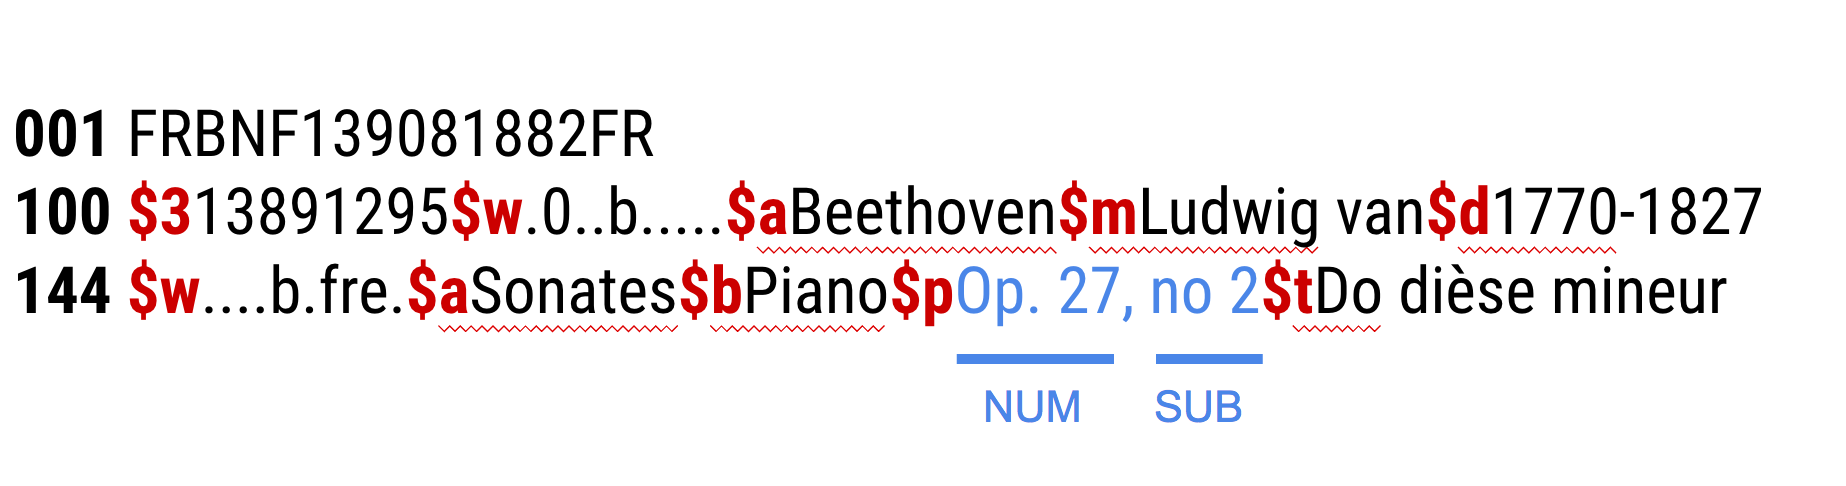
\includegraphics[width=6cm]{figs/MARC_example.png}}}
  \caption{An excerpt of a UNIMARC record.}
 \label{fig:unimarc}
 \smallskip
 \centerline{\framebox{
  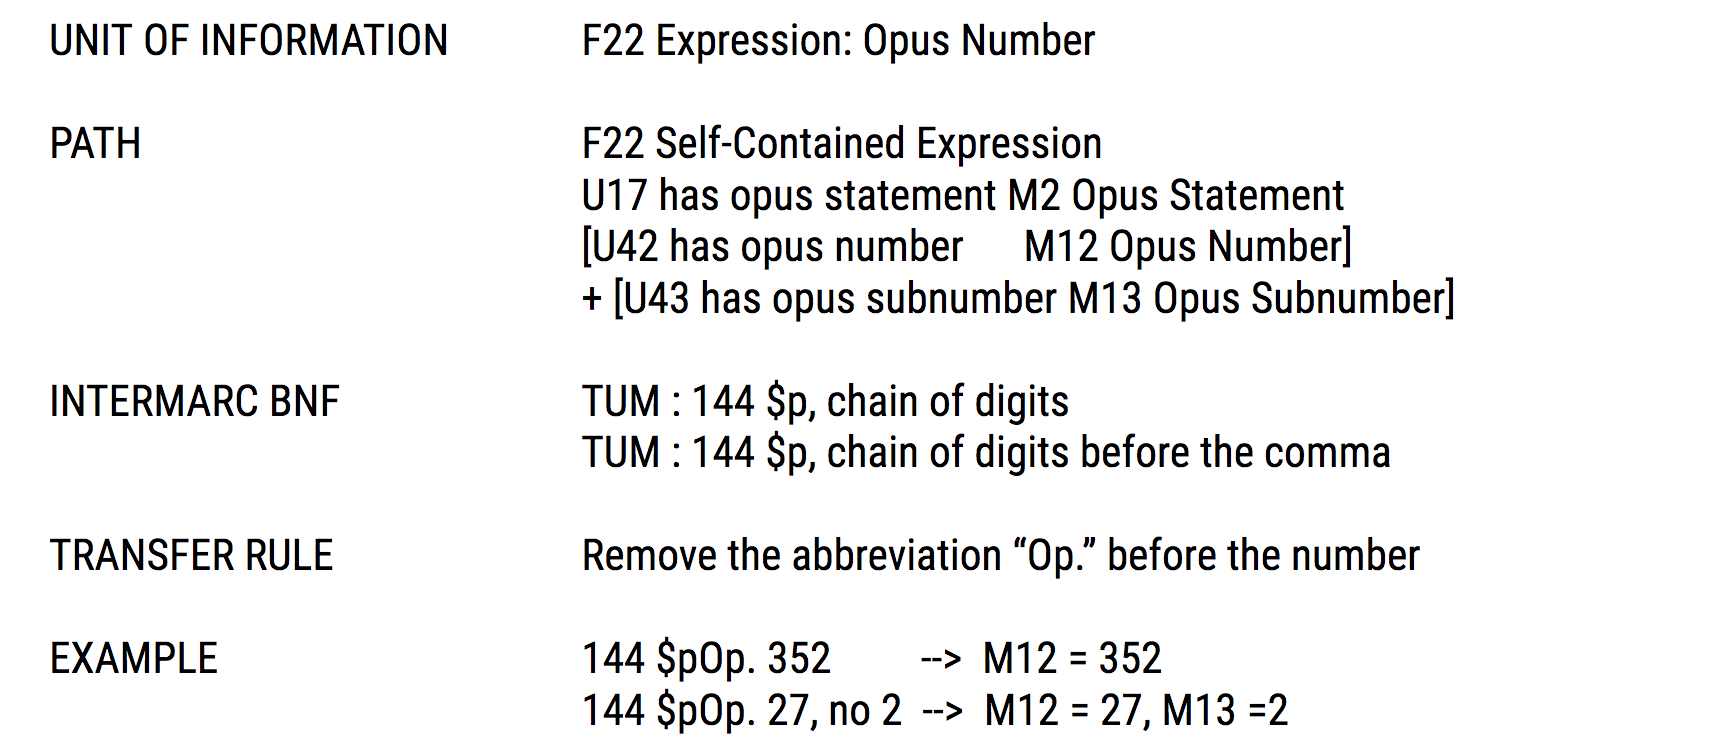
\includegraphics[width=\columnwidth]{figs/mapping_rule.png}}}
  \caption{Example of mapping rules describing the opus number and sub-number of a work}
 \label{fig:mappings}
\end{figure}

\begin{figure*}
 \centerline{
 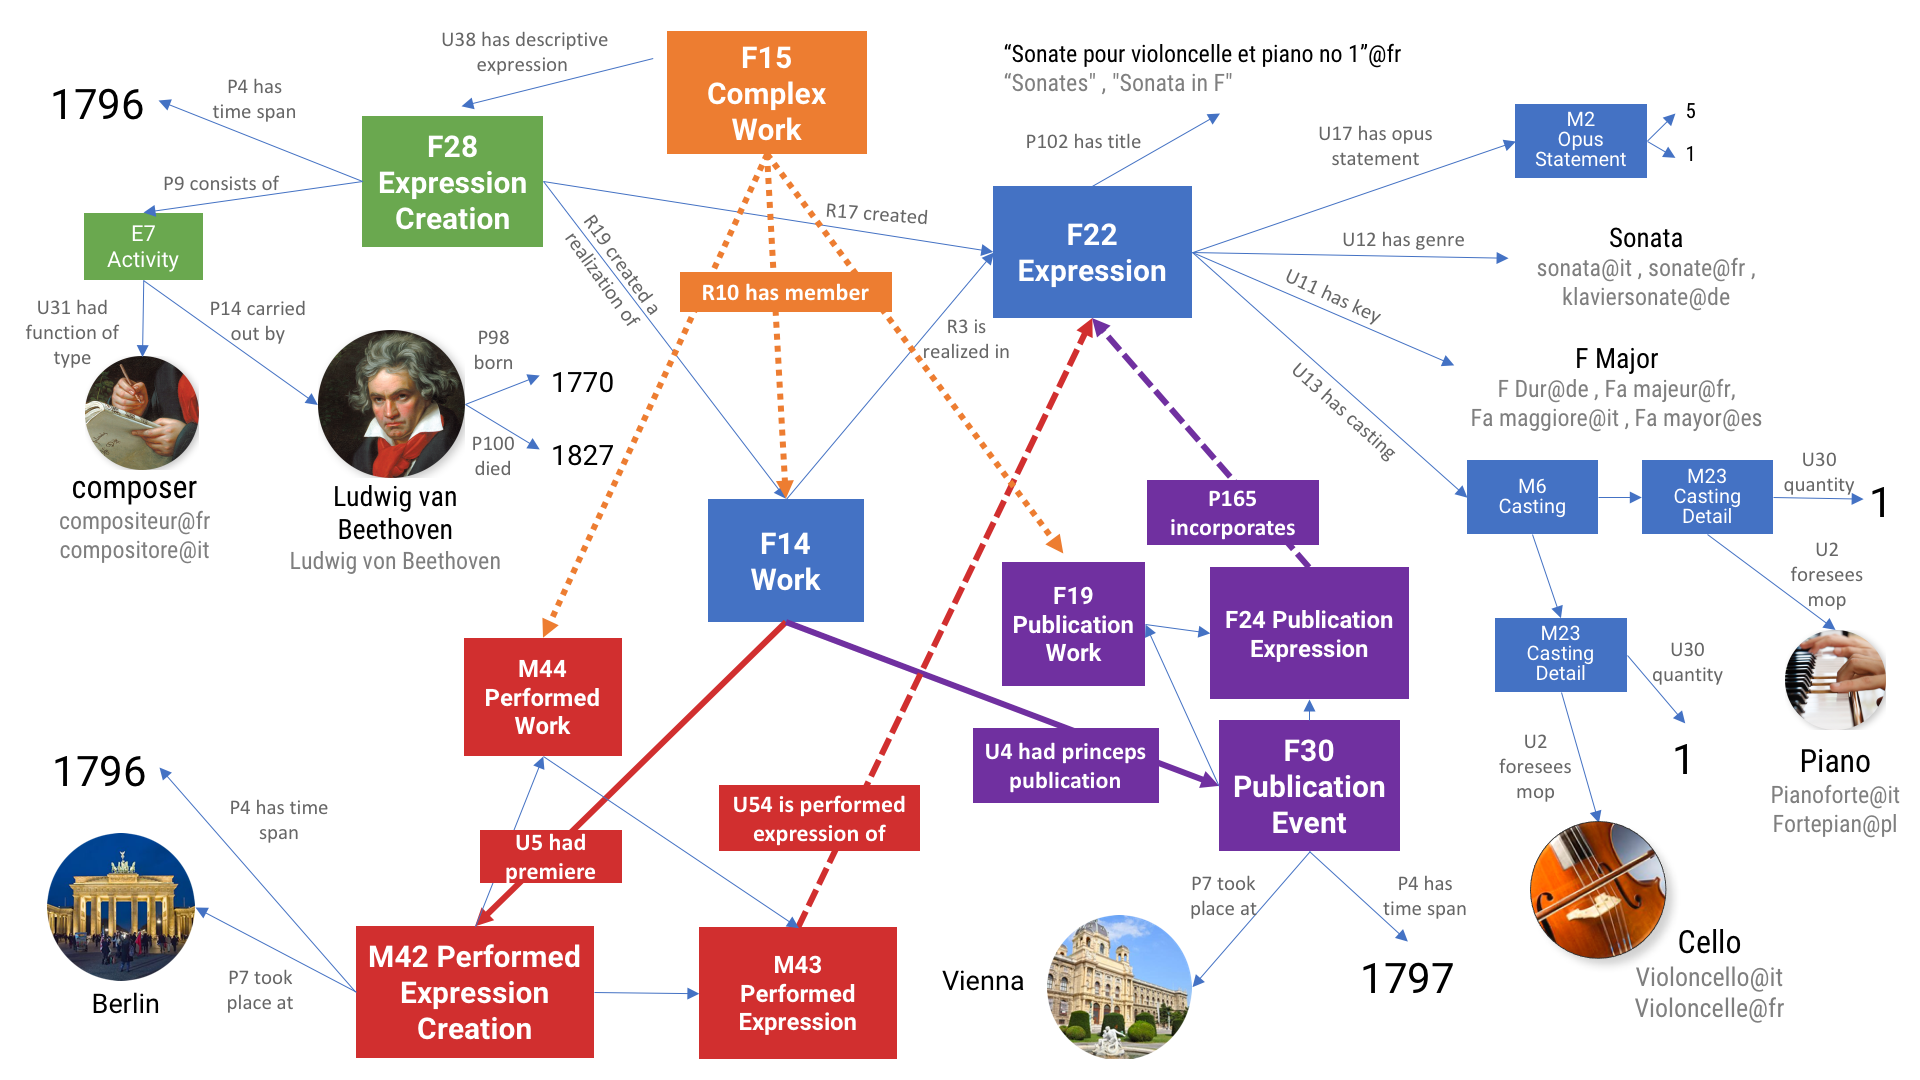
\includegraphics[width=\textwidth]{figs/schema_2.png}}
 \caption{Beethoven's \textit{Sonata for piano and cello n.1} represented as a graph}
 \label{fig:schema}
\end{figure*}

\subsection{Example as a Graph}
The graph depicted in \figref{fig:schema} shows a real example from our data: Beethoven's \textit{Sonata for piano and cello n.1}\footnote{\url{http://data.doremus.org/expression/614925f2-1da7-39c1-8fb7-4866b1d39fc7}}. The FRBRoo triplet contains all the information about the work and its composition. Then, the information about the performance and publication are linked to the triplet through specific properties. The nodes represented as circles consist normally in URIs taken from controlled vocabularies (the function ``composer'' or the genre ``sonata'') or are entities that are matched to external datasets (the person of Beethoven or the places Berlin and Vienna), that can have alternative labels (i.e. in different languages) and additional information. Each one of these nodes can represent a link between different works, performances, etc., making everything connected in a large graph.

We point out the modelling of the casting as a positive example of the expressiveness of the model that allows to declare all the MoPs required for a particular work and, for each of them, declare the foreseen quantity, the eventual responsibility of soloist for some of them, the interpreted role (for operas), etc.

\subsection{Data Linking} \label{subsec:datalinking}
If we take again the example of the BnF and the Philharmonie data providers, after the conversion process, we end up with two RDF graphs sharing a large number of entities, such as music works or creation events. Therefore, a crucial task in order to enable the interoperability between these datasets and to enable their exploration, is the task of data linking, defined as establishing the identity relations between the elements of these graphs in a (mostly) automated manner. First, we focus on matching music works across datasets. However, due to the high data heterogeneity in the musical field, link discovery becomes a challenging task. These heterogeneities include important structural, syntactic and lexical differences in descriptions of musical works, use of languages or titles, etc. To train and test data linking tools, we have collected benchmark data from these institutions as part of the 2016 OAEI instance matching evaluation campaign.\footnote{\url{http://islab.di.unimi.it/content/im_oaei/2016/##doremus}}

Our initial tests with off-the-shelf linking tools, such as SILK,\footnote{\url{http://silkframework.org}} did not show satisfactory results. We have, therefore, developed \textit{Legato}, a novel linking system based on the DOREMUS use case, designed to handle the heterogeneities of music data mentioned earlier. The processing pipeline of Legato consists in automatically pre-processing, comparing, repairing and providing a set of identity links (a link set). The system takes as an input a source and a target dataset. We sketch the algorithm unfolding in the following steps.
 
(i) Data cleaning. This step aims at ignoring what we call ``noisy'' properties, leading to errors, making it difficult to compare resources. Imagine the likely case of different data providers assigning different identifiers to equivalent resources across datasets (e.g., the records of a musical work in the catalogs of two libraries). Another common example are properties that contain comments in the form of long strings that cannot be safely directly compared. 

(ii) Instance profiling. This step allows to represent each resource by a sub-graph considered relevant for the comparison task;

(iii) Instance indexing and matching. These steps aim at generating a large pool of mapping candidates, guaranteeing high recall. Indexing techniques are applied on the resources allowing to represent them as textual documents containing the values of their properties collected at a given predefined depth of the RDF graph and considered relevant for the description of a resource. In that way, a work will be represented by a set of keywords coming from the RDF description of its resource. Note that we include the labels of resources identified by URIs in order to achieve a more complete description (e.g., the URI identifier of a music genre will be replaced by the literal containing its name in English). This allows to seamlessly compare instances in a way in which text documents are compared in a classical information retrieval framework.

(iv) Post-processing step. This step aims at reducing the false positives rate and increasing precision. Instances in each dataset are clustered by using a standard hierarchical clustering algorithm~\cite{rokach2005clustering}. Afterwards, pairs of matching clusters are identified across datasets using a metric function on the clusters centroids. Each pair of matching clusters is analyzed and compared on the basis of their properties. In order to improve the effectiveness of this comparison, we apply the key ranking algorithm RANKEY~\cite{achichi2016automatic}, allowing to identify the most suitable properties for the comparison. The resulting linkset is used to repair errors possibly produced at steps (ii) and (iii), helping to disambiguate highly similar, though distinct pairs of works, previously generated as candidates.

Note that \textit{Legato} is well-suited for users with little or no technical knowledge of the linking process, since it requires very little configuration, in contrast to most state-of-the-art tools \cite{nentwig2015survey}---only the classes of the instances to compare need to be explicitly indicated to the tool. 

%%%%%%%%%%%%%%%%%%%%%%%%%%%%%%%%%%%%%%%%%%
%%%  5. Music Discovery with Overture  %%%
%%%%%%%%%%%%%%%%%%%%%%%%%%%%%%%%%%%%%%%%%%

\section{Music Discovery with Overture}
\label{sec:exploration}
We developed the first version of \textsc{Overture} (Ontology-driVen Exploration and Recommendation of mUsical REcords), a prototype of an exploratory search engine for DOREMUS data. \textsc{Overture} is developed as a modern web app, implemented with Node.JS and Angular and available at \url{http://overture.doremus.org}. The application makes requests directly to our SPARQL endpoint\footnote{\url{http://data.doremus.org/sparql}} and provides the information in a nice user interface (UI).

\subsection{Visualizing the Complexity}
At the top of the user interface, the navigation bar allows the user to navigate between the main concepts of the DOREMUS model: expression, performance, score, recording, artist. The challenge is in giving to the final user a complete vision on the data of each class and letting him/her understand how they are connected to each other. \figref{fig:overture-detail} represents Beethoven's \textit{Sonata for piano and cello n.1}. Aside from the different versions of the title, the composer and a textual description, the page provides details on the information we have about the work, like the musical key, the genres, the intended MoP, the opus number. When these values come from a controlled vocabulary, a link is present in order to search for expressions that share the same value, for example, the same genre or the same musical key. A timeline shows the most important events in the story of the work (the composition, the premiere, the first publication). Other performances and publications can be represented below. 

The background is a portrait of the composer that comes from DBpedia. It is retrieved thanks to the presence in the DOREMUS database of \texttt{owl:sameAs} links. These links comes in part from the International Standard Name Identifier (ISNI) service\footnote{The ISNI database contains authority information about people involved in creative processes (i.e. artists). It is managed by the ISNI Quality Team, which the BnF is a member of, and artists record in the BnF database contains generally an ISNI reference.}, in part thanks to an interlinking realised by matching the artist name, birth and death date in the different datasets.

\begin{figure}
 \centerline{
 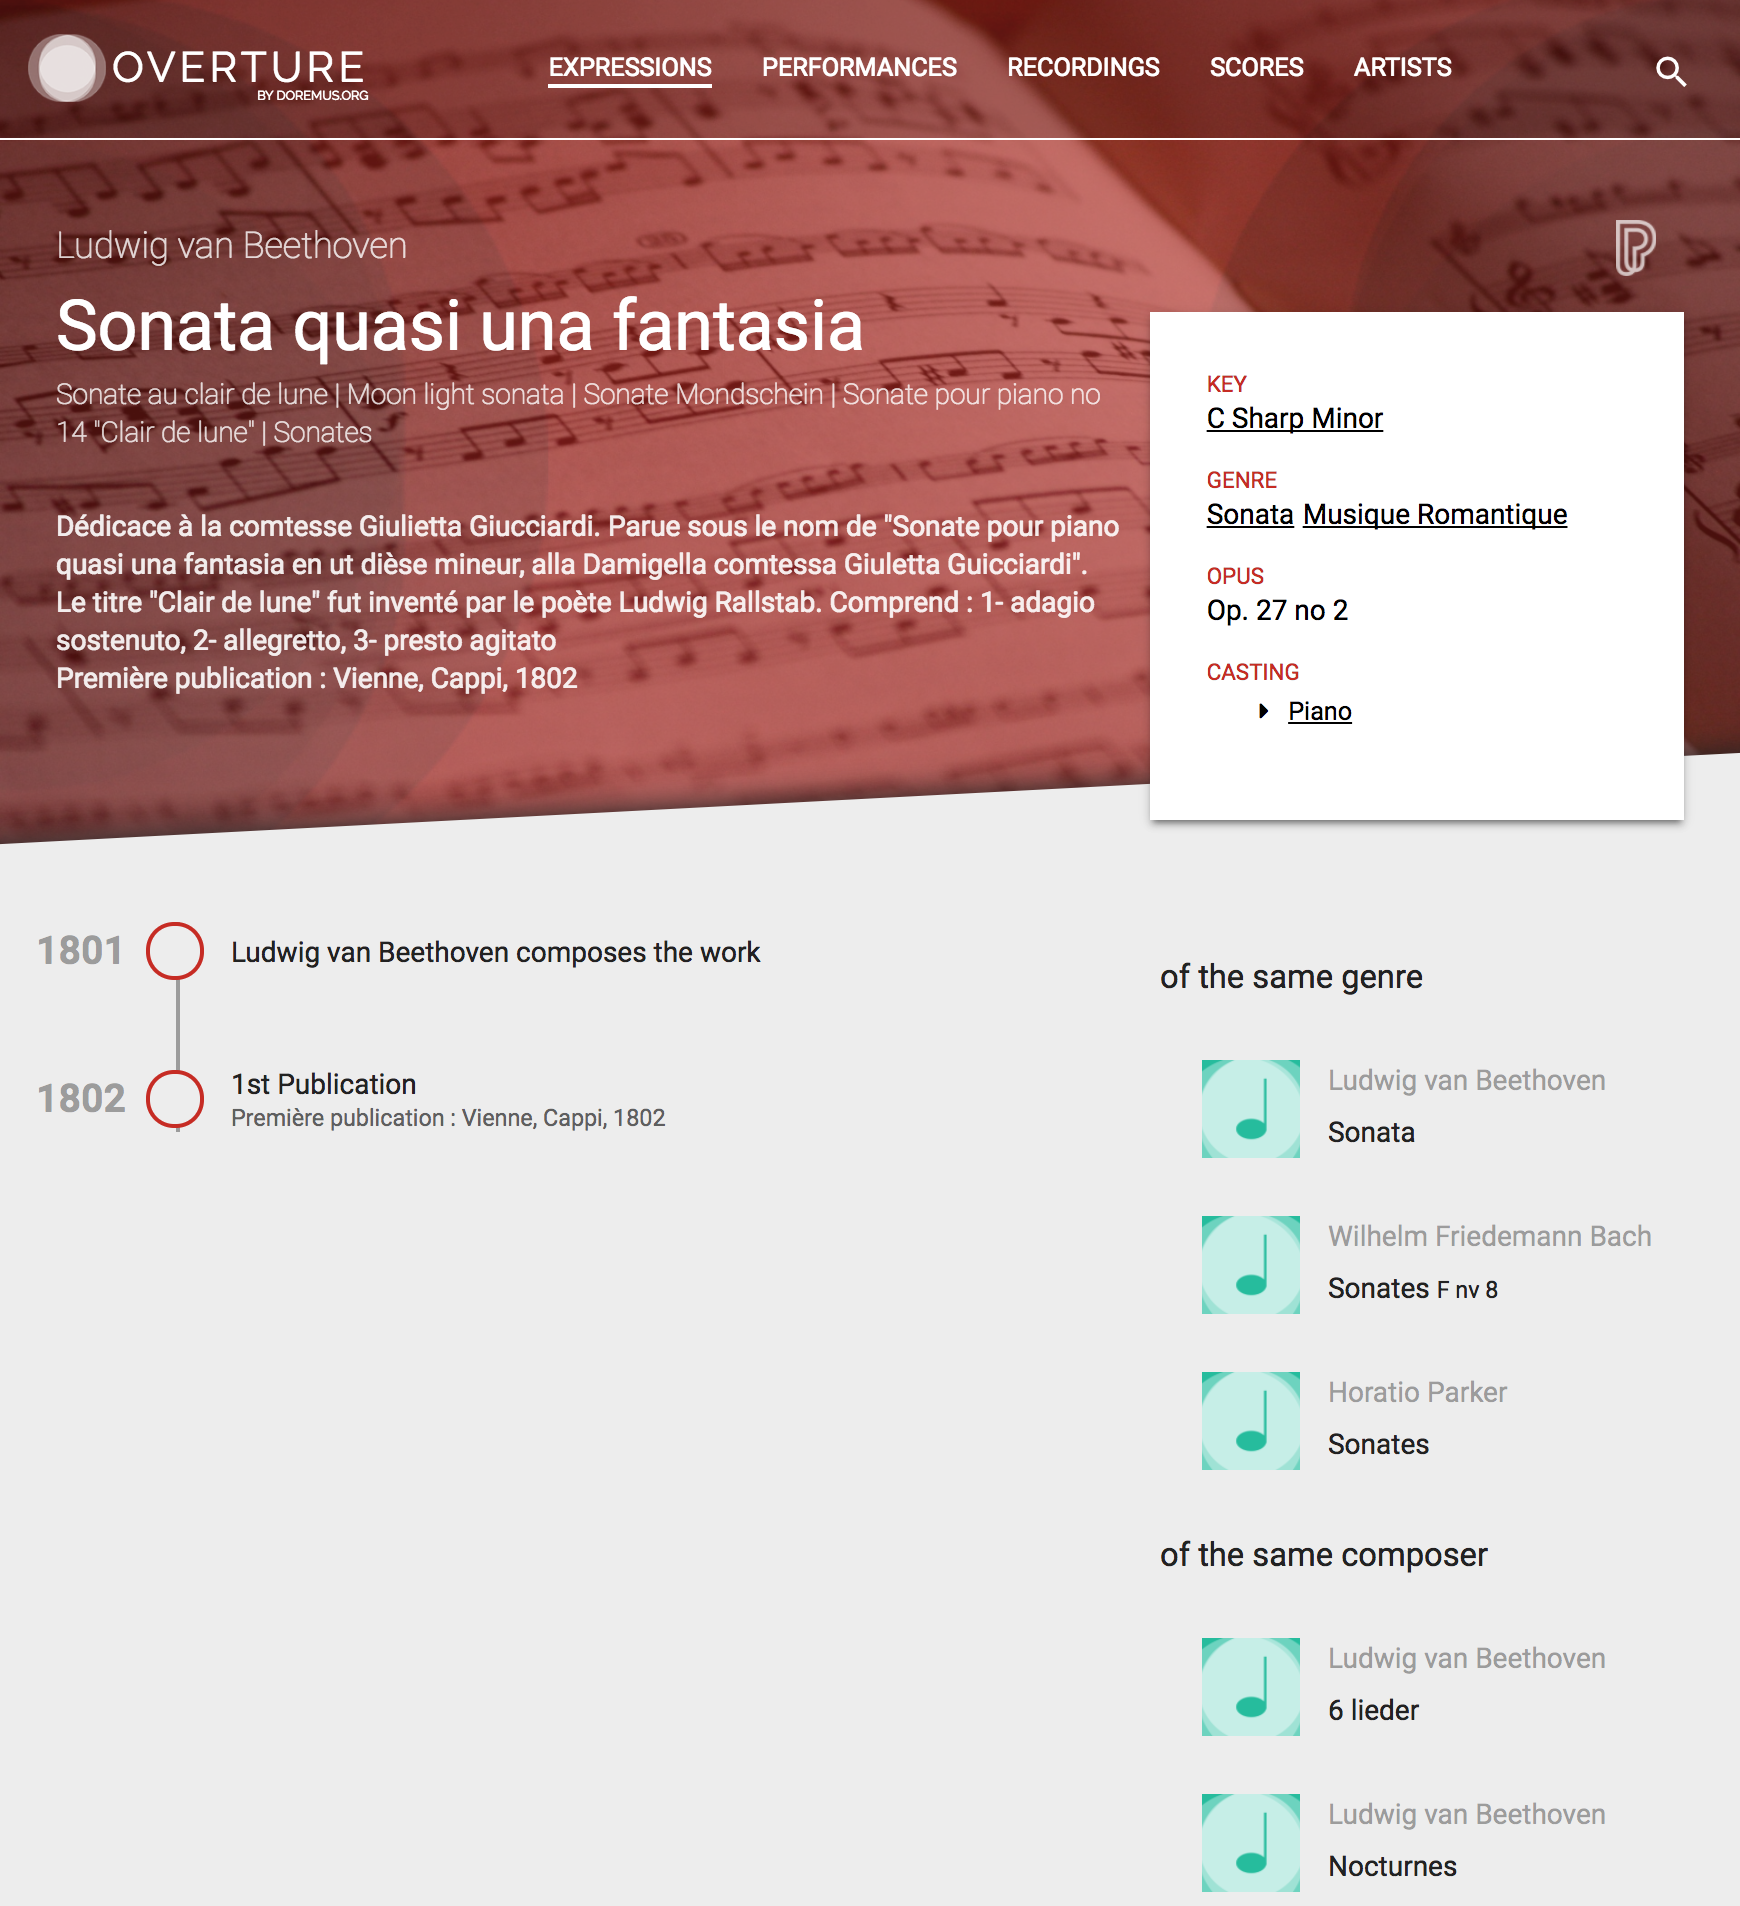
\includegraphics[width=\columnwidth]{figs/Overture_sonata.png}}
 \caption{The detail of an expression in \textsc{Overture}}
 \label{fig:overture-detail}
\end{figure}

\subsection{Explore and Recommend}
\begin{figure}
 \centerline{
 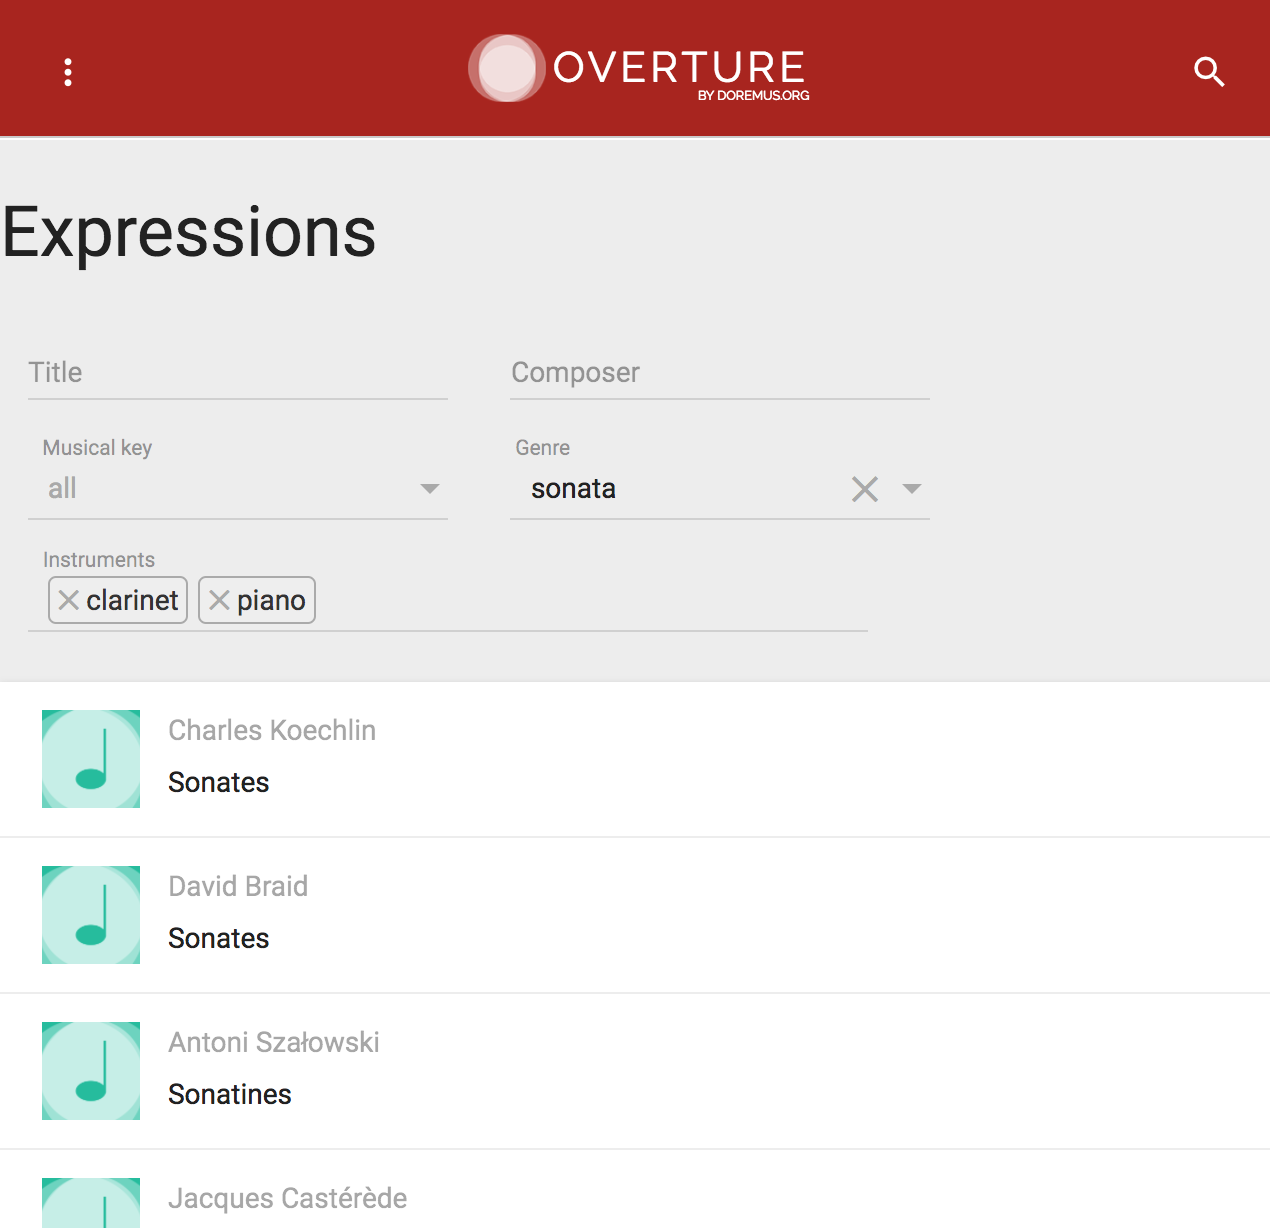
\includegraphics[width=\columnwidth]{figs/overture_list_2.png}}
 \caption{The list of expressions filtered by genre and MoP.}
 \label{fig:overture-list}
\end{figure}

The richness of the DOREMUS model offers to the end-user the chance to perform a detailed advanced search. All expressions are searchable by facets, that include the title and the composer, but also keys, genres, detailed castings, making it possible to select very precise subsets of data, like all the sonatas (genre) that involves a clarinet and a piano (MoPs) \figref{fig:overture-list}. The hierarchical properties in the controlled vocabulary allow the smart retrieval not only of the entity that match exactly the chosen value (i.e. \textit{Strings, bowed}), but also any of its narrower concepts (i.e. \textit{violin}, \textit{cello}, etc.).

An alternative way to discover the information in \texttt{Overture} is to follow links in every page of the application. Passing from an expression to its movements, from an artist to its works and from a performance to its recordings, will let the user explore the data following the links in the same way they are in the graph. Also, certain properties can work as a bridge between entities, appearing clickable in the user interface.

We inserted a very simple recommendation section in the expression page, that suggests other expressions that have some properties in common with the current one, like the genre, the composer and the foreseen instruments. This part will host in the future more sophisticated recommendation, that automatically brings the user to new interesting elements, similar to the one currently displayed, enabled by the richness of the data and the structure of RDF.

%%%%%%%%%%%%%%%%%%%%%%%
%%%  6. Evaluation  %%%
%%%%%%%%%%%%%%%%%%%%%%%

\section{Evaluation}
\label{sec:evaluation}
In this section, we provide an evaluation of our model and of our linking tool {\it Legato}.

\subsection{Model Evaluation}
The success of a model can be evaluated in its ability in providing answers to end-user questions. Before the beginning of the project, a list of questions have been collected from experts of the partner institutions\footnote{\url{https://github.com/DOREMUS-ANR/knowledge-base/tree/master/query-examples}}. These questions reflect real needs of the institutions and involves problems that they face daily in the task of selecting information from the database (e.g. concert organisation or broadcast programming) or for supporting librarian and musicologist studies. They can be related to practical use cases (the search of all the scores that suit a particular formation), to musicologist topics (the music of a certain region in a particular historical period), to interesting stats (the works usually performed or published together), or to curious connections between works, performances or artists. Most of the questions are very specific and complex, so that it is very hard to find their answer by simply querying the search engines currently available on the web. We have grouped these questions in categories, according to the DOREMUS classes involved in the question. We translated them into SPARQL queries that we run on the DOREMUS endpoint. We can distinguish 4 different cases:

(i) Questions that fit perfectly the model and the data and that can be readily converted as SPARQL queries (e.g. \textit{Retrieve all performances in which a composer interprets his or her works}, that is also represented in \figref{fig:sparql-question});

(ii) Questions that fit the model but not yet the current state of the data since data conversion is still a work in progress. It is sometimes difficult to parse the source files when they contain plain text and not a regular syntax that enables to extract structured information (e.g. \textit{Retrieve the list of the works of which at least one of the dedicatees is also a performer of the work}, when the data about dedication are not yet in our dataset);

(iii) Questions that overflow the model, because they contain aspects that go beyond the music information and involve other kind of knowledge. An example is \textit{Retrieve a list of works of chamber music composed in the 19\textsuperscript{th} century by Scandinavian composers}: it requires to know the birth place of the composer, and if this place is located in one of the Scandinavian countries;

(iv) Questions with an intrinsic complexity (e.g. \textit{Retrieve the works written for -- strictly / at least / at most -- violin, clarinet and piano}). Most of them are caused by the nature of the Semantic Web, that includes an Open World Assumption, and makes hard the formulation of queries that involves the check for the absence of a certain property. Despite this, we can anyway provide an answer to this query by considering only information contained in our database (Closed World Assumption).

Regarding the case (iii), we can state that these are very interesting questions, because they are the ones that can fully exploit the advantages of linked data technologies. In fact, this kind of queries are quite far from having an answer in a traditional data storing system (e.g. database). The vocation of the Web of Data in interconnecting the knowledge gives the possibility of performing federated queries involving the Linked Open Data cloud (LOD) and in particular datasets such as Geonames or DBpedia. For this reasons, the interconnection of the data is crucial. 

\begin{figure}
 \centerline{ \framebox{
  
\includegraphics[width=6cm]{figs/question.png}
  }}
  \smallskip
 \centerline{ \framebox{
 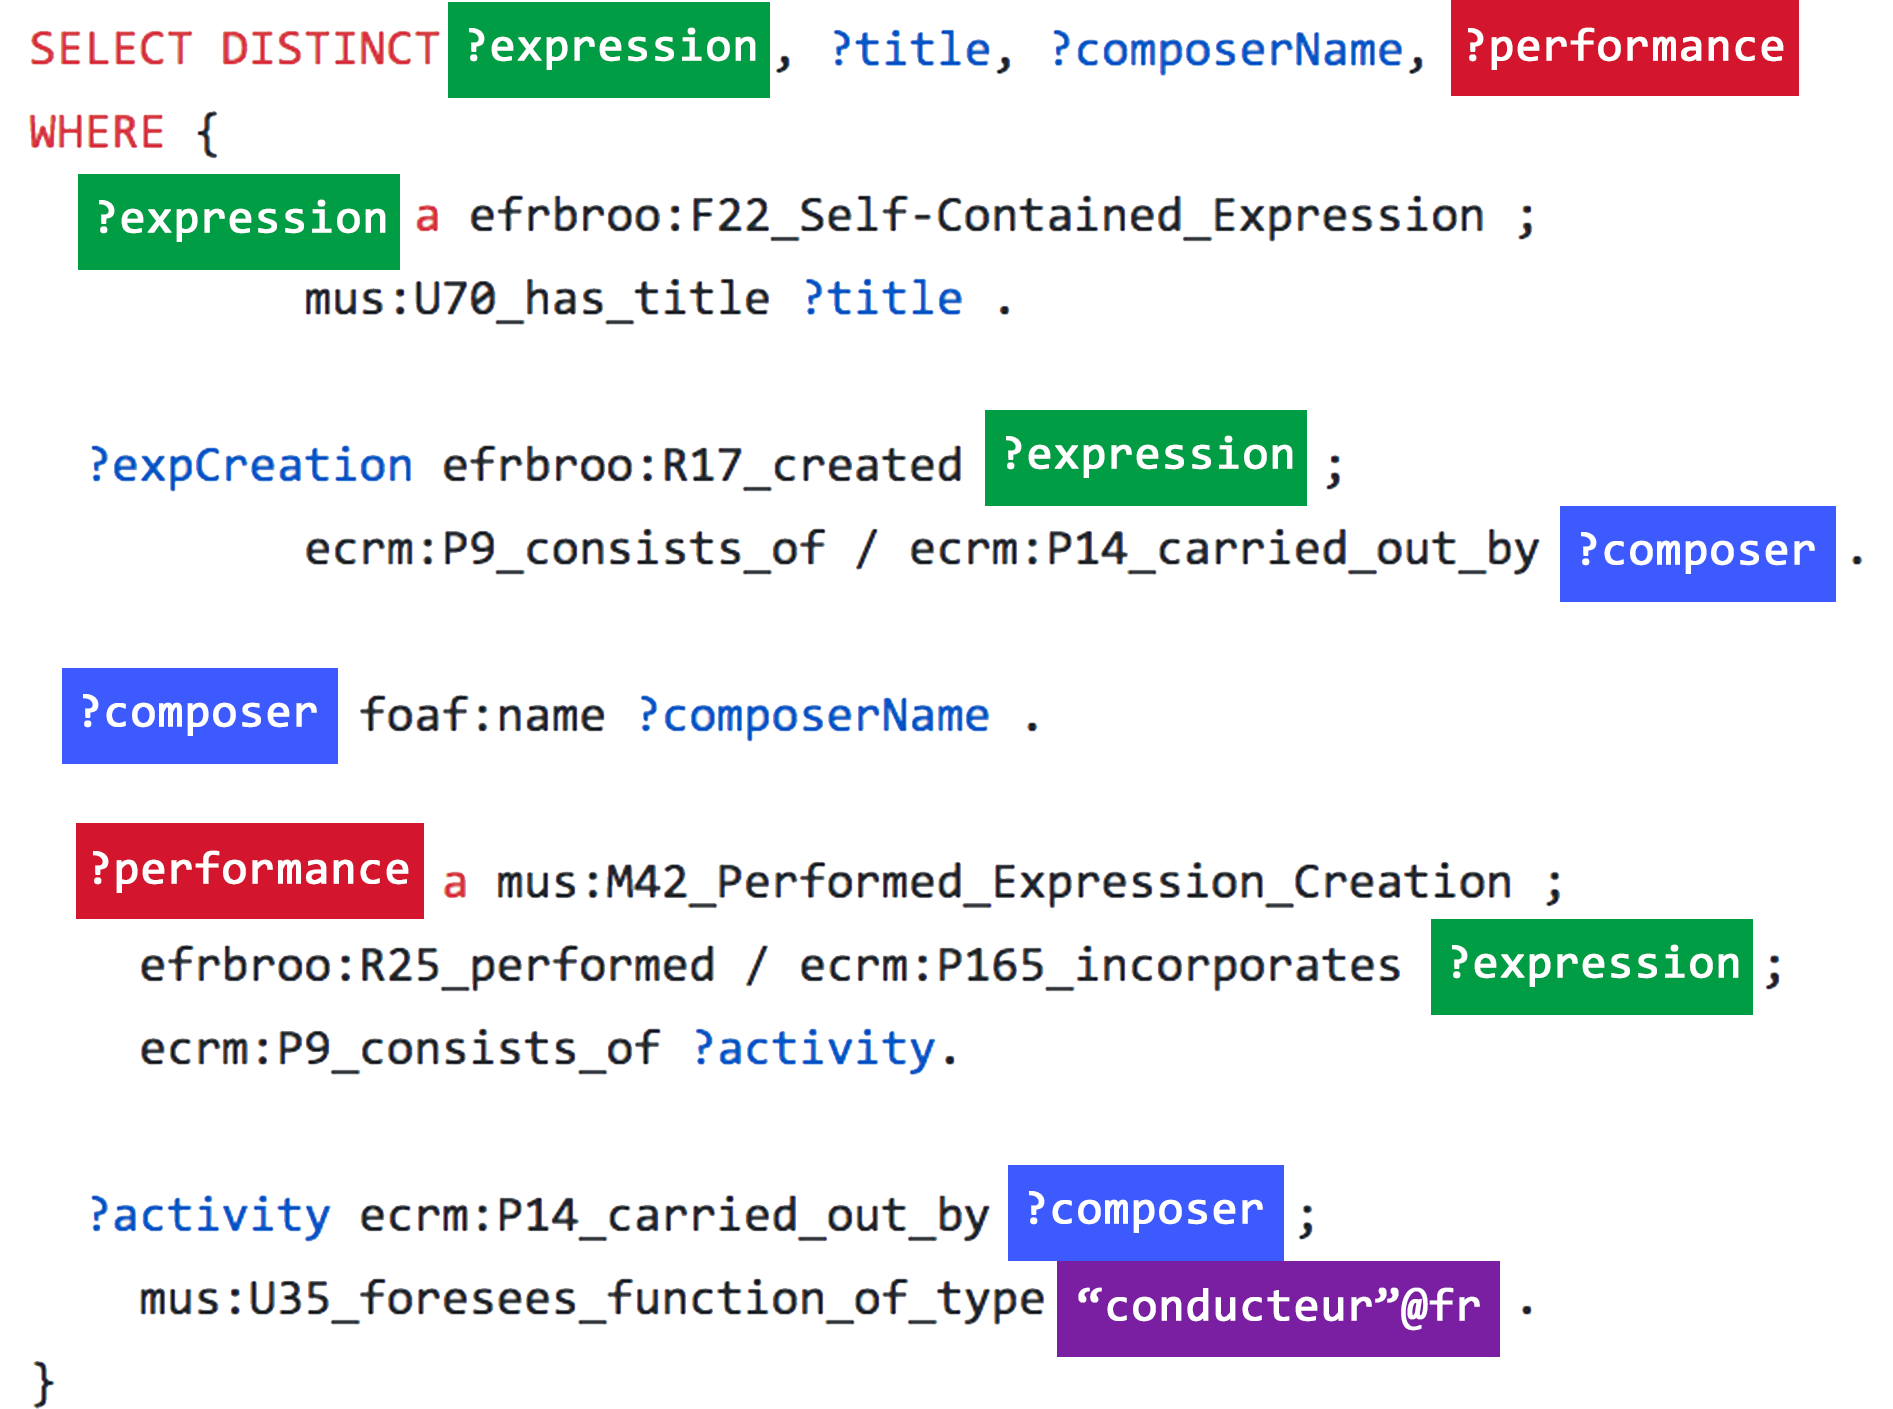
\includegraphics[width=\columnwidth]{figs/sparql.png}
 }}
 \caption{A natural language question and its SPARQL query version. The colored boxes shows logically related parts.}
 \label{fig:sparql-question}
 
\end{figure}

\tabref{tab:queries} provides an overview of how many queries we can currently write for each category. The implementation of recordings, scores, performance that is still work in progress -- along with the interconnection to the LOD repositories -- is one important reason for which some questions have not yet been translated into SPARQL and other ones have not results. 

\begin{table}
 \begin{center}
 \begin{tabular}{|l|c|}
  \hline
  Category & Query~/~Questions \\
  \hline
  A. Works & 23 / 29 \\
  \hline
  B. Artists & 1 / 3 \\
  \hline
  C. Performances & 6 / 9 \\
  \hline
  D. Recordings & 0 / 11 \\
  \hline
  E. Publications & 0 / 5 \\
  \hline
 \end{tabular}
\end{center}
 \caption{For each category of questions, we provide the ratio of the number of converted queries}
 \label{tab:queries}
\end{table}

% TODO integrate this queries in Overture.

\subsection{Linking with \textit{Legato}} \label{sec:eval-link}
\begin{table*}[t]
\begin{center}
	\begin{tabular}{|c|c|c|c|c|c|c|c|c|c|}
		\hline
		{}{}{} & \multicolumn{3}{c|}{9-HT} & %
		\multicolumn{3}{c|}{4-HT} &  \multicolumn{3}{c|}{FP-trap}\\
		\cline{2-10}
		& F & P & R & F & P & R & F & P & R \\
		\hline
		\textbf{\textbf{\textit{Legato}}} & 0.92 & 0.93 & 0.9 & 0.88 & 0.89 & 0.87 & 0.85 & 0.87 & 0.82 \\
		\hline
		\textbf{SILK} & 0.6 & 0.76 & 0.5 & - & - & - & 0.31 & 0.34 & 0.29\\
		\hline
	\end{tabular}
	\caption{Results on the DOREMUS benchmark data from the OAEI's instance matching track 2016}
	\label{table:doremus}
\end{center}
\end{table*}

We have evaluated the performance of our linking tool \textit{Legato} (Section~\ref{subsec:datalinking}) by comparing it to a state-of-the-art tool, SILK, on the DOREMUS benchmark data that was published on the Instance Matching track of OAEI 2016 campaign. Note that although the DOREMUS data has evolved since the publication of this benchmark, this evaluation is done on the publicly available OAEI datasets. This track consists of three datasets, described below. 

Nine heterogeneities (9-HT): This dataset consists of two small graphs from the BnF and the Philharmonie, containing about 40 instances each. The linking task consist in discovering 1:1 equivalence relations between them. There are 9 types of heterogeneities that these data manifest, that have been identified by the music library experts, such as multilingualism, differences in catalogs, differences in spelling, different degrees of richness of description, etc.

Four heterogeneities (4-HT): This track consists of two bigger datasets containing about 200 instances each, related by 1:1 equivalence relations. There are 4 types of heterogeneities that these datasets manifest: 1) Orthographic differences, 2) Multilingual titles, 3) Missing properties, 4) Missing titles.

The False Positives Trap (FP-trap): This task consists in correctly disambiguating the instances contained in two datasets, by discovering 1:1 equivalence relations between the instances that they contain. We have selected several groups of works with highly similar descriptions where there exist only one correct match in each group. The goal is to challenge the linking tools capacity to avoid the generation of false positives and match correctly works in the presence of highly similar but still distinct candidates.

SILK needs to be configured by pointing out the properties to use for the linking. Therefore, we have first run a key selection and ranking algorithm, allowing to select automatically the properties that provide the best likelihood of discovering links between two datasets, as described in~\cite{achichi2016automatic}. We have then used these properties to configure SILK, thus providing the ``best conditions'' for the tool to perform. The results of the comparison in terms of F-measure, Precision and Recall are given in Table \ref{table:doremus}. As we can see from the table, \textit{Legato} outperforms SILK on all three tasks (no results are returned by SILK on the second task). 

%%%%%%%%%%%%%%%%%%%%%%%%%%%%%%%%%%%%%%%
%%%  7. Conclusion and Future Work  %%%
%%%%%%%%%%%%%%%%%%%%%%%%%%%%%%%%%%%%%%%

\section{Conclusion and Future Work}
\label{sec:conclusion}
We proposed a complete workflow for the management of music metadata using Semantic Web technologies. We developed a specialized ontology and a set of controlled vocabularies for the different concepts specific to music. Then, we proposed an approach for converting and interlinking data, in order to go beyond the librarian practice currently in use. Finally, we show how these data can be used in a real web application, allowing the end-user to explore the data and get music recommendation.

As future work, once the validation of vocabulary alignment will be completed, we will produce a pivot vocabulary for each category, that contains all the concepts and the different labels that come from the different sources, in order to connect the entire knowledge graph. On the data side, we are working on the improvement of the parsing of the data using Named Entity Recognition (NER) techniques, that will link also the DOREMUS data to external LOD datasets, like DBpedia, Wikidata and MusicBrainz. Regarding the data linking task, although our results on the benchmark data are promising, we still need to address several scaling issues that will allow us to efficiently interconnect our datasets, containing sometimes hundreds of thousands of records. We will be also working on creating links from our data to well-established web knowledge graphs, such as DBpedia.

Finally, we are planning to integrate a series of interesting features in \textsc{Overture}, which include the integration of media like images and sound tracks, the retrieving of related information from LOD, and the realisation of a dashboard with interesting and unusual results (along the lines of the Wikipedia homepage). Moreover, a content-based recommendation system will be developed in order to exploit the richness of DOREMUS data. The recommendation results will be available through API and hosted in the web application.

%%%%%%%%%%%%%%%%%%%%%%%%%%%%
%%%  8. Acknowledgments  %%%
%%%%%%%%%%%%%%%%%%%%%%%%%%%%

\section{Acknowledgments}
This work has been partially supported by the French National Research Agency (ANR) within the DOREMUS Project, under grant number ANR-14-CE24-0020.

\bibliographystyle{ACM-Reference-Format}
\bibliography{bib-doremus} 

\end{document}
